\runningheader{SAT Mathematics}{Drill Set 12}{Page \thepage\ of \numpages}

\begingradingrange{sat-drill-12}
\subsection*{SAT Drill 12}

\question[1]
If $6n + 40 = 3(2n - 20) + 2n$, what is the value of $2n$?
\begin{solution}
100
\end{solution}

\question[1]
The game store sells both board games and figurines. Board games sell for $\$40$ a game and figurines sell for $\$15$ a figurine. If the store sells 80 total pieces of merchandise and earned $\$2625$ from those sales, how many board games did the game store sell?
\begin{choices}
  \choice 23
  \choice 40
  \choice 48
  \CorrectChoice 57
\end{choices}

\question[1]
The equation $nA = 360$ shows the relationship between the measure $A$, in degrees, of an exterior angle of a regular polygon and $n$, the number of sides of the polygon. If a regular polygon's exterior angle is greater than 80 degrees, what is the greatest number of sides it can have?
\begin{choices}
  \CorrectChoice 4
  \choice 5
  \choice 6
  \choice 8
\end{choices}


\newpage





\question[1]
A study asked voluntary participants to record the number of cups of water they drink in a month and the electric bill for the month. The results are shown in the scatterplot. What can be inferred from the scatterplot?
\begin{center}
  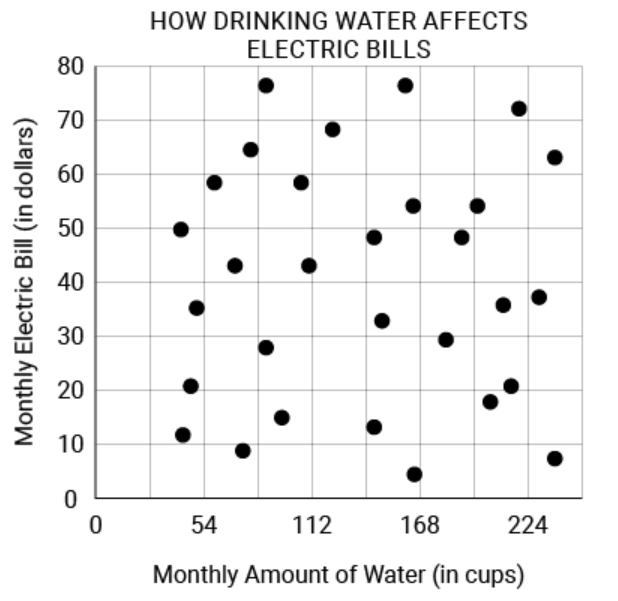
\includegraphics[width=0.90\linewidth]{images/cus29}
\end{center}
\begin{choices}
  \choice No one drinks less than 27 cups of water in a month.
  \choice The more water one drinks, the higher the electric bill.
  \choice There is no correlation between the monthly amount of water drunk and the electric bill.
  \choice Drinking bottled water explains why some electric bills are lower.
\end{choices}

\question[1]
A right triangle has legs with lengths of 15 centimeters and 25 centimeters. If the length of this triangle's hypotenuse, in centimeters, can be written in the form $5\sqrt{n}$, where $n$ is an integer, what is the value of $n$?
\begin{solution}
34
\end{solution}





\newpage





\question[1]
The graph of line $q$ is shown. Line $r$ is perpendicular to line $q$. What is the slope of line $r$?
\begin{center}
  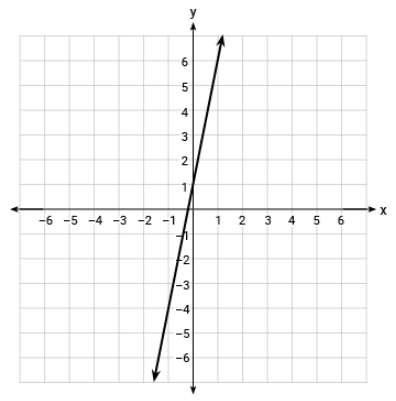
\includegraphics[width=0.90\linewidth]{images/cus30}
\end{center}
\begin{choices}
  \choice $-5$
  \choice $-\frac{1}{5}$
  \choice $\frac{1}{5}$
  \choice $5$
\end{choices}

\question[1]
For the linear function $g(x)$, $g(2.6) = 11$ and $g(5) = 3.8$. When graphed on the coordinate plane, the function $g(x)$ is perpendicular to the graph of the linear function $h(x) = m x$. What is the value of $m$?
\begin{choices}
  \choice $-3$
  \choice $-\frac{1}{3}$
  \CorrectChoice $\frac{1}{3}$
  \choice $3$
\end{choices}






\newpage





\question[1]
Harold prepared a sample of bacteria. A strain of virus killed 30 percent of the bacteria, but within a week, the surviving population had grown 47 percent. Which of the following represents the value of the original population in terms of the new population $p$?
\begin{choices}
  \choice $\frac{p}{1.17}$
  \choice $1.17p$
  \CorrectChoice $\frac{p}{(0.70)(1.47)}$
  \choice $(0.70)(1.47)p$
\end{choices}

\question[1]
The population of fruit flies in a laboratory study triples every 7 days. The population at the beginning of the study numbered 200. Which equation represents the population of fruit flies, $y$, in the study $t$ weeks after the beginning of the study?
\begin{choices}
  \CorrectChoice $y = 200(3)^t$
  \choice $y = 3(200)^t$
  \choice $y = 200(3)^{\frac{t}{7}}$
  \choice $y = 200^{3t}$
\end{choices}

\question[1]
Consider the system:
\[
  \begin{gathered}
  24 x+24 y=-8 y+\frac{2}{3} \\
  -k y=3 x-\frac{1}{12}
  \end{gathered}
\]
In the given system of equations, $k$ is a constant. If the system has infinite solutions, what is the value of $k$?
\begin{solution}
4
\end{solution}






\newpage





\question[1]
As a probe descends to the Kuril Trench in the Pacific Ocean, it records the amount of dissolved oxygen in the water in parts per million (ppm). At depths below 2,000 meters, the dissolved oxygen drops at a constant rate of $d$ ppm for every change in depth of 100 meters until it reaches zero. At a depth of 2,530 meters, the dissolved oxygen is measured to be 205 ppm. At a depth of 3,030 meters, the dissolved oxygen is measured to be 65 ppm. What is the value of $d$?
\begin{solution}
28
\end{solution}

\question[1]
Mrs. Brennan wants to buy $x$ computers for her company and has a budget of $B$ dollars. If she buys $x$ computers today, they will cost $\$1,000$ each, and she will need to raise an additional $\$2,000$. If she waits two months, the computers will cost $\$900$ each, and she will have $\$400$ left over. What is the value of $B$?
\begin{choices}
  \choice 14,800
  \choice 21,600
  \CorrectChoice 22,000
  \choice 24,000
\end{choices}

\question[1]
Let $f(x) = x(x-14) + 70 - k$, where $k$ is an integer constant. For which of the following values of $k$ will the graph of the function have no $x$-intercepts?
\begin{choices}
  \CorrectChoice 20
  \choice 21
  \choice 25
  \choice 30
\end{choices}

\question[1]
A professional football team practices 6 days a week in the preseason. A water boy for the team knows that the players drink about 200 gallons of water each day of preseason practice. If the water tank in the utility room pours water at a rate of 9 gallons per minute, how many hours a week does the water boy spend filling water containers?
\begin{choices}
  \choice $\frac{10}{27}$
  \CorrectChoice $\frac{20}{9}$
  \choice $\frac{100}{27}$
  \choice $\frac{400}{3}$
\end{choices}

\question[1]
The graph of $x^2 + 3x + y^2 - y = \frac{13}{2}$ in the $xy$-plane is a circle. What is the length of the circle's radius?
\begin{solution}
3
\end{solution}

\question[1]
Consider the equation:
\[
  3(a x + b) = \frac{21}{10}x - \frac{48}{11}
\]
In the given equation, $a$ and $b$ are constants and $b > 0$. The equation has no solution. What is the value of $a$?
\begin{solution}
$\frac{7}{10}$
\end{solution}






\newpage





\question[1]
Which expression is equivalent to $\frac{1}{\frac{1}{x+5} + \frac{1}{x-2}}$?
\begin{choices}
  \choice $\frac{2}{2x+3}$
  \choice $\frac{2x+3}{2}$
  \choice $\frac{2x+3}{x^2+3x-10}$
  \CorrectChoice $\frac{x^2+3x-10}{2x+3}$
\end{choices}

\question[1]
The box plot summarizes the values in two different data sets. Based on the box plot, which of the following must be true?
\begin{center}
  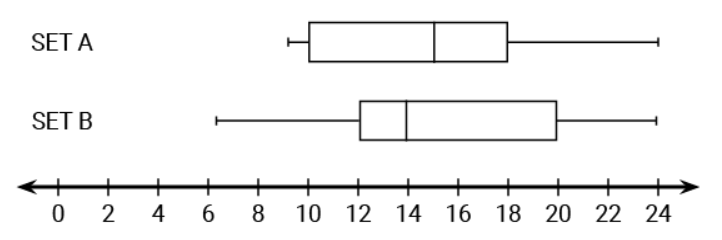
\includegraphics[width=0.90\linewidth]{images/cus31}
\end{center}
\begin{choices}
  \choice The mean of set $A$ is greater than the mean of set $B$.
  \choice The range of set $A$ is greater than the range of set $B$.
  \choice The median of set $A$ is greater than the median of set $B$.
  \choice The standard deviation of set $A$ is greater than the standard deviation of set $B$.
\end{choices}

\question[1]
How many distinct real solutions does the equation $0.6x^2 - 1.5x + 2.01 = 0$ have?
\begin{choices}
  \CorrectChoice Zero
  \choice Exactly one
  \choice Exactly two
  \choice Infinitely many
\end{choices}






\newpage





\question[1]
A regular hexagon is inscribed in a rectangle as shown.
\begin{center}
  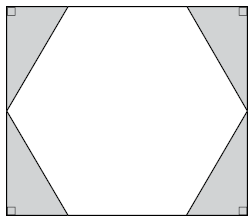
\includegraphics[width=0.70\linewidth]{images/cus32}
\end{center}
The perimeter of the hexagon is $6a$ units. What is the area of the shaded region, in square units?
\begin{choices}
  \choice $\frac{\sqrt{3}}{8}a^2$
  \choice $\frac{\sqrt{3}}{2}a^2$
  \choice $\frac{3\sqrt{3}}{2}a^2$
  \choice $2\sqrt{3}a^2$
\end{choices}

\question[1]
The function $g(x)$ is defined as $g(x) = (x^2 + bx + c)(x + a)$, where $a$, $b$, and $c$ are constants. There are two distinct values such that $g(x) = 0$. If $g(x)$ can also be written in the form $\frac{1}{m}(mx^2 + mbx + b^2)(x + a)$, what is the value of $m$?

\textbf{Note}: $-a$ must be one of the two distinct answers.
\begin{solution}
4
\end{solution}






\newpage





\question[1]
The function $f$ is defined by the equation $f(x) = \frac{x}{a-9}$, where $a$ is a positive constant and $a \neq 9$. If the value of the product of $f(2a)$ and $f(18a)$ is equal to $\frac{9}{100}$, what is the value of $a$?
\begin{solution}
$\frac{3}{7}$
\end{solution}

\question[1]
Angela buys 2 cookies and 3 brownies for a total of $\$19$. Vicky buys 4 cookies and 1 brownie for a total of $\$13$. If $c$ represents the cost of a cookie and $b$ represents the cost of a brownie, which system of equations can determine the cost of one cookie and one brownie?
\begin{choices}
  \choice
  \[
    \begin{aligned}
    & c+b=5 \\
    & 6c+4b=32
    \end{aligned}
  \]
  \CorrectChoice
  \[
    \begin{aligned}
    & 2c+3b=19 \\
    & 4c+b=13
    \end{aligned}
  \]
  \choice
  \[
    \begin{aligned}
    & 5c=19b \\
    & 5b=13c
    \end{aligned}
  \]
  \choice
  \[
    \begin{aligned}
    & 6c=19 \\
    & 4b=13
    \end{aligned}
  \]
\end{choices}

\question[1]
Which expression is equivalent to $x^2 + 5x - 6$?
\begin{choices}
  \choice $(x+2)(x-3)$
  \choice $(x-2)(x+3)$
  \choice $(x+1)(x-6)$
  \CorrectChoice $(x-1)(x+6)$
\end{choices}






\newpage





\question[1]
A circle in the $xy$-plane has its center at $(-3,7)$, and the point $(1,7)$ lies on the circle. Which equation represents this circle?
\begin{choices}
  \choice $(x-3)^2 + (y+7)^2 = 4$
  \choice $(x+3)^2 + (y-7)^2 = 4$
  \choice $(x-3)^2 + (y+7)^2 = 16$
  \CorrectChoice $(x+3)^2 + (y-7)^2 = 16$
\end{choices}

\question[1]
The graph of line $a$ is shown, and the equation of line $a$ is $y=3x+1$. Line $b$ is parallel to line $a$ and crosses through the points $(0,5)$ and $(k,-7)$. What is the value of $k$?
\begin{center}
  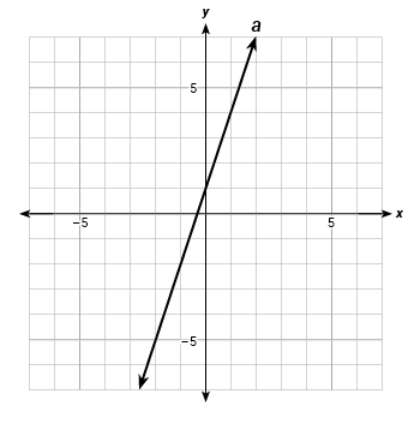
\includegraphics[width=0.90\linewidth]{images/cus33}
\end{center}
\begin{solution}
-4
\end{solution}






\newpage





\question[1]
A linear inequality is graphed on the $xy$-coordinate plane. Which coordinate point is a solution to the graphed inequality?
\begin{center}
  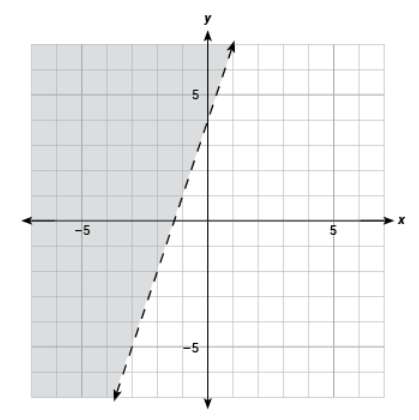
\includegraphics[width=0.70\linewidth]{images/cus34}
\end{center}
\begin{choices}
  \CorrectChoice $(-3,-4)$
  \choice $(-2,-3)$
  \choice $(0,4)$
  \choice $(1,6)$
\end{choices}

\question[1]
Data set $X$: $25$, $32$, $11$, $42$, $33$, $16$, $27$, $39$, $54$.

If 54 is removed from the data set, which of the following is true?
\begin{choices}
  \choice The mean and the median do not change.
  \choice The mean and the median change by the same amount.
  \choice The change to the median is greater than the change to the mean.
  \CorrectChoice The change to the mean is greater than the change to the median.
\end{choices}

\question[1]
What is one of the solutions to the equation $2x^2 - 40x + 182 = 0$?
\begin{solution}
7
\end{solution}






\newpage





\question[1]
How many solutions does the equation $2(37x+1) = 37(2x+1)$ have?
\begin{choices}
  \choice Exactly one
  \choice Exactly two
  \choice Infinitely many
  \CorrectChoice Zero
\end{choices}

\question[1]
The scatterplot shows the comparison for the time and the cost to hire a plumber. At what hour is the predicted cost the closest to an actual cost to hire a plumber?
\begin{center}
  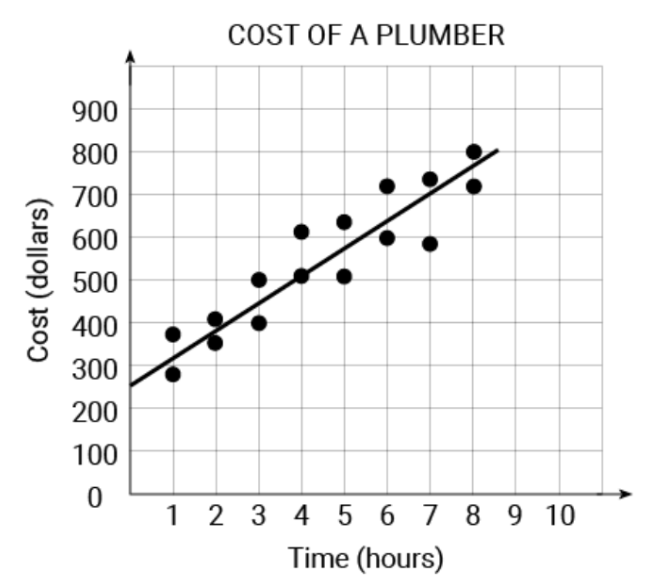
\includegraphics[width=0.90\linewidth]{images/cus35}
\end{center}
\begin{solution}
4
\end{solution}






\newpage





\question[1]
Two linear equations $m$ and $n$ are graphed on the $xy$-coordinate plane, as shown. If line $m$ is perpendicular to line $n$, what is the value of the $y$-intercept of line $n$?
\begin{center}
  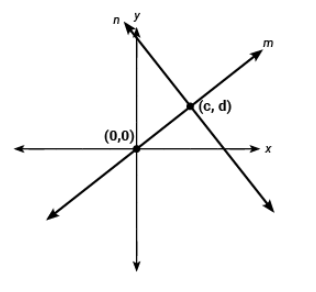
\includegraphics[width=0.90\linewidth]{images/cus36}
\end{center}
\begin{choices}
  \choice $d-\frac{c^2}{d}$
  \CorrectChoice $d+\frac{c^2}{d}$
  \choice $d-\frac{d^2}{c}$
  \choice $d+\frac{d^2}{c}$
\end{choices}

\question[1]
In certain conditions, filamentous fungi will grow exponentially, tripling in size every day. If, on day 1, the fungi are each 4 mm in length, which of the functions below represents the length on the $n^{\text{th}}$ day?
\begin{choices}
  \choice $y=3(4)^n$
  \choice $y=3(4)^{n-1}$
  \choice $y=4(3)^n$
  \CorrectChoice $y=4(3)^{n-1}$
\end{choices}






\newpage





\question[1]
In the equation $2x^2 - 27x + d = 0$, $d$ is a positive integer constant. The equation has no real solutions. What is the smallest possible value for $d$?
\begin{choices}
  \choice 91
  \CorrectChoice 92
  \choice 93
  \choice 94
\end{choices}

\question[1]
The equation $m^6 = (n+5p)^3$ relates the variables $m, n$, and $p$ for all real numbers $>0$. Which equation correctly expresses $n$ in terms of $m$ and $p$?
\begin{choices}
  \choice $n=\sqrt[3]{m^3-5p}$
  \choice $n=m^2-\sqrt[3]{5p}$
  \CorrectChoice $n=m^2-5p$
  \choice $n=m^3-5p$
\end{choices}

\question[1]
In the right triangle $ABC$, angle $C$ is a right angle. If $\cos(A) = \frac{x-k}{x+k}$, where $k$ is a constant and $x$ is the side length of $BC$, what is the value of $x$ in terms of $k$?
\begin{choices}
  \choice $2k$
  \CorrectChoice $4k$
  \choice $2k^2$
  \choice $4k^2$
\end{choices}






\newpage





\question[1]
The table shows the price for ordering different quantities of shirts. A delivery fee is calculated as a percentage of the base cost of the shirts. Then, a tax is applied to the combined cost of the shirts and the delivery.
\begin{center}
  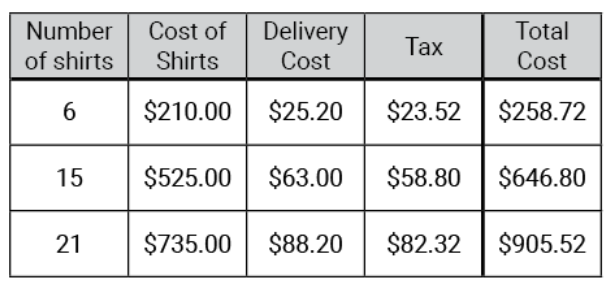
\includegraphics[width=0.90\linewidth]{images/cus37}
\end{center}
If $p$ is the percentage added for delivery and $q$ is the percentage added for taxes, what is the value of $p-q$?
\begin{choices}
  \choice 0.8
  \choice 2
  \choice 6.67
  \choice 23.2
\end{choices}

\question[1]
A cruise ship charges $\$4$ per soda for the first 19 sodas and then charges $\$2.50$ for each additional soda. If $c(s)$ is the total cost, in dollars, for $s$ sodas and $s>19$, what is the equation of $c(s)$?
\begin{choices}
  \choice $c(s) = 2.5s + 19$
  \CorrectChoice $c(s) = 2.5s + 28.5$
  \choice $c(s) = 2.5s + 76$
  \choice $c(s) = 6.5s + 47.5$
\end{choices}






\newpage





\question[1]
The exponential function $f(x)$ is graphed on the $xy$-plane. The function $g(x)$ (not shown) is defined such that $g(x) = f(x-1) + k$. If $g(0) = 1$, what is the value of $k$?
\begin{center}
  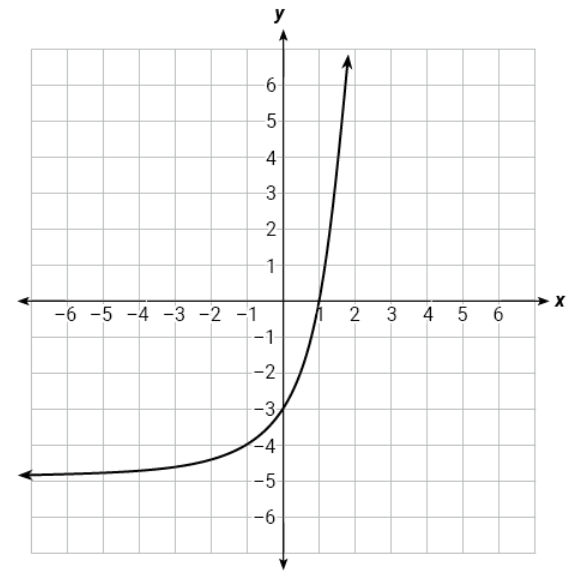
\includegraphics[width=0.90\linewidth]{images/cus38}
\end{center}
\begin{choices}
  \choice $-5$
  \choice $-4$
  \choice $4$
  \CorrectChoice $5$
\end{choices}

\question[1]
Line $A: y=ax+b$ and line $B: y=cx+d$, where $a, b, c, d$ are constants and $b>d$, intersect in the first quadrant of the $xy$-coordinate plane at the point $(j, k)$. A triangle is formed from the $y$-intercepts of the lines and the point of intersection, and the base is formed by the distance between the $y$-intercepts of the lines. If the base and height of the triangle are equal, what is the value of $c-a$?
\begin{solution}
1
\end{solution}






\newpage





\question[1]
A rectangular pyramid has a base length measuring $b$ centimeters, a base width measuring $2b$ centimeters, and a height measuring $c$ centimeters, as shown. A similar rectangular pyramid has side lengths that are all $\frac{2}{3}$ the side lengths of the given rectangular pyramid. What is the volume of the smaller rectangular pyramid?
\begin{center}
  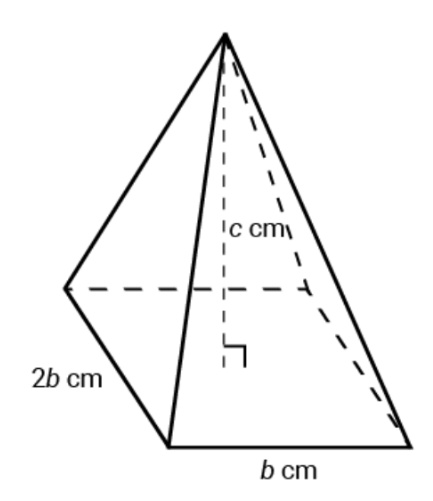
\includegraphics[width=0.55\linewidth]{images/cus39}
\end{center}
\begin{choices}
  \choice $\frac{2b^2c}{3}$
  \choice $\frac{4b^2c}{9}$
  \choice $\frac{8b^2c}{27}$
  \CorrectChoice $\frac{16b^2c}{81}$
\end{choices}

\question[1]
A quadratic equation intercepts the $x$-axis at two different points, $(0,0)$ and $(2j, 0)$, where $j>0$. The distance between the $x$-intercepts is equal to the shortest distance from the $x$-axis to the vertex, and the vertex is in the first quadrant. Which of the following represents the quadratic equation?
\begin{choices}
  \choice $y=\frac{2}{3j}(x)(x-2j)$
  \choice $y=-\frac{2}{3j}(x)(x-2j)$
  \choice $y=-\frac{j}{2}(x)(x-2j)$
  \CorrectChoice $y=-\frac{2}{j}(x)(x-2j)$
\end{choices}






\newpage





\question[1]
For the quadratic equation $kx^2 - 62x + 288 = 0$, if the product of the solutions is $-72$, what is the value of $k$?
\begin{solution}
-4
\end{solution}

\question[1]
Circle $O$ has its center at point $O$, as shown. Points $A, B$, and $C$ lie on Circle $O$ and $AB$ is the diameter. Triangle $ACB$ is inscribed in the circle, and altitude $CD$ is shown. The length of $CB=7$ centimeters and $AC=\sqrt{95}$ centimeters. Which of the following is closest to the ratio of $CB$ to $CD$?
\begin{center}
  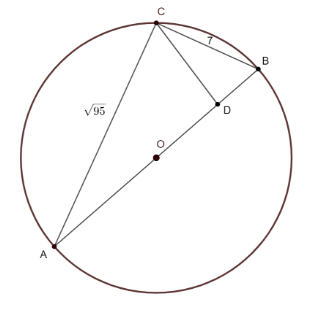
\includegraphics[width=0.72\linewidth]{images/cus40}
\end{center}
\begin{choices}
  \choice $1.7:1$
  \choice $1.4:1$
  \CorrectChoice $1.2:1$
  \choice $1.1:1$
\end{choices}

\endgradingrange{sat-drill-12}
